% Rapport de résultats -- Métadonnées, ETL / ELT et capture des changements
% Compilation : xelatex rapport.tex (deux fois) ; pdflatex fonctionne aussi si babel-french est installé.
% Images dans captures/.
% Les passages en rouge entre crochets sont à compléter par le membre indiqué.
\documentclass[10pt,a4paper]{article}
\usepackage{iftex}
\ifPDFTeX
  \usepackage[utf8]{inputenc}
  \usepackage[T1]{fontenc}
  \usepackage{lmodern}
  \usepackage[french]{babel}
\else
  \usepackage{fontspec}
  \usepackage{polyglossia}
  \setmainlanguage{french}
\fi
\usepackage[a4paper,margin=2cm]{geometry}
\usepackage{microtype}
\usepackage{xcolor}
\usepackage{booktabs,tabularx,array}
\usepackage{enumitem}
\usepackage{graphicx}
\usepackage{float}
\usepackage{caption}
\usepackage{titlesec}
\usepackage[hidelinks]{hyperref}

\captionsetup{font=small,labelfont=bf}
\setlist{noitemsep,topsep=2pt,leftmargin=1.3em}
\setlength{\parindent}{0pt}
\setlength{\parskip}{3pt}
\renewcommand{\arraystretch}{1.12}
\titleformat{\section}{\large\bfseries}{\thesection.}{0.5em}{}
\titleformat{\subsection}{\normalsize\bfseries}{\thesubsection}{0.5em}{}
\titlespacing*{\section}{0pt}{9pt}{3pt}
\titlespacing*{\subsection}{0pt}{6pt}{2pt}
\newcommand{\todo}[1]{\textcolor{red}{[#1]}}

\begin{document}

\begin{center}
  {\LARGE\bfseries Rapport de résultats}\\[2pt]
  {\large Métadonnées, ETL / ELT et capture des changements}\\[4pt]
  Erdem Ertan \textperiodcentered{} Bekir Uzumcu \textperiodcentered{} Eray Aksoy\\
  Université de Galatasaray --- 3 novembre 2026
\end{center}

%==========================================================================
\section{Synthèse de l'article et lien avec notre projet}

\subsection{L'article en bref}

\paragraph{Problème.} Mekterovi\'c, Brki\'c et Baranovi\'c~\cite{mekterovic2011} partent d'un constat : les tests des procédures ETL sont écrits sur mesure pour chaque entrepôt et se réutilisent très peu. Ils proposent une procédure générique de test d'intégration dont la question centrale est « \emph{all counts match} » : les données extraites ont-elles bien été chargées, et sont-elles exactes ? La qualité visée est l'exactitude et la fiabilité entre les sources relationnelles et l'entrepôt ; les erreurs déjà présentes dans la source sont hors périmètre.

\paragraph{Méthode.} L'ETL est traité comme une boîte noire : on compare seulement ses entrées et ses sorties, en trois points (sources SRC, zone de staging SA, entrepôt DW). Un système de test, qui ne fait que lire, comprend un sous-système de comptage (CS : combien d'enregistrements manquent ou sont en trop ?) et un sous-système de différences (DS : lesquels ?). Hypothèses : un entrepôt dimensionnel, des sources relationnelles, et chaque fait traçable vers un seul enregistrement source (tables agrégées et instantanés exclus).

\paragraph{Lignage.} Une dimension contient déjà la clé métier (BK). Pour une table de faits, où les clés étrangères sont remplacées par des clés de substitution, l'article ajoute une clé $SK_{FT}$ et une table de lignage $linFt=\{SK_{FT},BK\}$, remplie au chargement au moyen d'une table temporaire scindée en deux projections. Deux requêtes génériques en découlent : les enregistrements manquants (présents dans la source filtrée $st'$, absents de l'entrepôt) et les enregistrements en trop (clés sans équivalent dans la source, ou faits sans entrée dans $linFt$).

\paragraph{Segmentation et comptage.} Comparer de gros ensembles est coûteux : la segmentation compte par groupes (typiquement année $\rightarrow$ mois $\rightarrow$ jour) et ne « fore » que les segments en désaccord, ce qui donne un filtre de sélection. Un COUNT seul laisse passer des erreurs qui s'annulent ; on ajoute d'autres agrégats (SUM). Le CS suit les comptages d'un chargement à l'autre (seuil : nouveau comptage $>t\times$ comptage précédent) ; en chargement incrémental, seules les données incrémentales sont segmentées.

\paragraph{CDC (section~6, tableaux~4 et~5).} Avec une dimension de type~2, les comptages de la source et de la dimension diffèrent légitimement : un \emph{update} ajoute une ligne (tableau~5). Ces écarts attendus sont journalisés (tables rDiff : clé métier, clé de substitution, cause) pour ne pas être pris pour des erreurs ; les tables iDiff recensent les enregistrements manquants ou en trop.

\paragraph{Étude de cas et limites.} Sur l'entrepôt HEIS (Croatie), la procédure a détecté des écarts dans 9~tables sur 89 ; la cause était une incompatibilité de plages de dates entre la source Informix et SQL Server~2000 (dates antérieures à 1753). Limites annoncées : deux hypothèses (modèle dimensionnel, sources relationnelles), une vérification partielle (comptages et montants de base) et une mise en œuvre partielle (CS de la phase extraction/CDC).

\subsection{Lien avec notre projet}

\paragraph{La procédure s'applique-t-elle à notre data mart ?} Oui, avec des nuances. Sur le chemin ELT (AdventureWorks $\rightarrow$ \texttt{stg} $\rightarrow$ \texttt{dm}), les trois points de comparaison existent : la méthode s'applique pleinement. Sur le chemin ETL, il n'y a pas de zone de staging (les transformations se font en mémoire avec pandas) : on ne dispose que de deux points, AdventureWorks et \texttt{dm}, et l'application est partielle.

\paragraph{Lignage.} Pour la dimension, \texttt{DimProduit} conserve \texttt{ProductID} et \texttt{CodeProduit} (clé métier). Pour les faits, l'énoncé prévoit déjà les colonnes \texttt{NumCommande} et \texttt{NumLigne} ; nous en avons fait la clé primaire de \texttt{FaitVente}, soit (\texttt{SalesOrderID}, \texttt{SalesOrderDetailID}), la clé métier de la ligne source. Le lignage est donc contenu dans la table de faits : c'est une adaptation de l'article, qui rend la table $linFt$ inutile.

\paragraph{Tableau~5 et nos règles de gestion.} Le tableau suivant confronte les effets des opérations à la source décrits par l'article à nos règles.

\smallskip
\begingroup\small
\begin{tabularx}{\textwidth}{@{}>{\raggedright\arraybackslash}p{3.6cm}>{\raggedright\arraybackslash}p{4.6cm}X@{}}
\toprule
Opération à la source & Tableau~5 de l'article & Notre règle \\
\midrule
Insert & Insert dans les dimensions et les faits & Nouveau produit : première version ; nouvelle ligne de commande : ligne de fait \\
Update d'un attribut SCD~2 (prix, sous-catégorie) & Dimension de type~2 : \textbf{Insert} & Clôture de la version courante et ouverture d'une nouvelle version \\
Update d'un attribut SCD~1 (nom) ou d'une ligne de commande & Dimension de type~1 : Update ; faits : Update & Nom écrasé dans toutes les versions ; fait mis à jour (quantité, montant) \\
Delete d'une ligne de commande & Faits : Delete ou None & Fait supprimé, nombre de suppressions journalisé (choix : Delete) \\
\bottomrule
\end{tabularx}
\endgroup

Nos règles sont cohérentes avec le tableau~5. Le Delete d'une ligne de dimension n'est pas exercé par le scénario.

\paragraph{Limites pour notre projet et ce qu'il faudrait ajouter.}
\begin{itemize}
  \item \emph{Chemin ETL :} pour appliquer pleinement la méthode, il faudrait matérialiser un jeu de données intermédiaire ; à défaut, on compare directement la source et \texttt{dm}.
  \item \emph{Versions SCD~2 :} comparer des clés métier ne vérifie pas que chaque fait est rattaché à la bonne version de produit. Il faut compléter par un test sur les intervalles de validité (\texttt{DateDebut}, \texttt{DateFin}), ce qui est précisément l'enjeu du produit~P (sections~4 à~6).
  \item \emph{Écarts attendus :} \texttt{meta.JournalChargement} conserve les comptages par exécution (lignes lues, insérées, mises à jour, supprimées, rejetées), ce qui rappelle le suivi du CS ; il ne détaille pas, comme les tables rDiff, la clé et la cause de chaque écart.
  \item \emph{CDC et Change Tracking :} l'article raisonne sur un CDC générique et ne distingue pas les deux mécanismes de SQL Server.
\end{itemize}

%==========================================================================
\section{Conception du data mart, métadonnées et règles SCD}

\subsection{Modèle et grain}

Le processus métier est la vente et le grain est une ligne de commande (une ligne de \texttt{Sales.SalesOrderDetail}). Les deux bases, \texttt{DM\_Ventes\_CDC} et \texttt{DM\_Ventes\_CT}, ont les mêmes schémas \texttt{dm} (trois tables) et \texttt{meta} ; \texttt{DM\_Ventes\_CT} contient en plus le schéma \texttt{stg}, copie brute de cinq tables sources pour l'ELT.

\noindent\begin{minipage}[t]{0.60\textwidth}
\vspace{0pt}\small
\begin{tabularx}{\linewidth}{@{}>{\raggedright\arraybackslash}p{2.1cm}X@{}}
\toprule
Table & Contenu \\
\midrule
\texttt{DimDate} & Clé \texttt{CleDate} (AAAAMMJJ) ; \texttt{Date}, \texttt{Annee}, \texttt{Trimestre}, \texttt{Mois}, \texttt{NomMois}, \texttt{Jour}, \texttt{JourSemaine}. Une ligne par jour du 2010-01-01 au 2030-12-31 (7\,670 lignes), générée en Python. \\
\addlinespace
\texttt{DimProduit} & Clé \texttt{CleProduit} (IDENTITY) ; \texttt{ProductID}, \texttt{CodeProduit}, \texttt{Nom}, \texttt{SousCategorie}, \texttt{Categorie}, \texttt{PrixCatalogue}, \texttt{DateDebut}, \texttt{DateFin}, \texttt{EstCourant}. Contraintes : \texttt{DateFin} $>$ \texttt{DateDebut} ; \texttt{EstCourant} = 1 si et seulement si \texttt{DateFin} est NULL ; index unique filtré (une seule version courante par produit). \\
\addlinespace
\texttt{FaitVente} & Clé (\texttt{NumCommande}, \texttt{NumLigne}) ; \texttt{CleDate}, \texttt{CleProduit} (clés étrangères), \texttt{Quantite}, \texttt{PrixUnitaire}, \texttt{Montant} $=$ \texttt{Quantite} $\times$ \texttt{PrixUnitaire}. \\
\bottomrule
\end{tabularx}
\end{minipage}\hfill
\begin{minipage}[t]{0.37\textwidth}
\vspace{0pt}
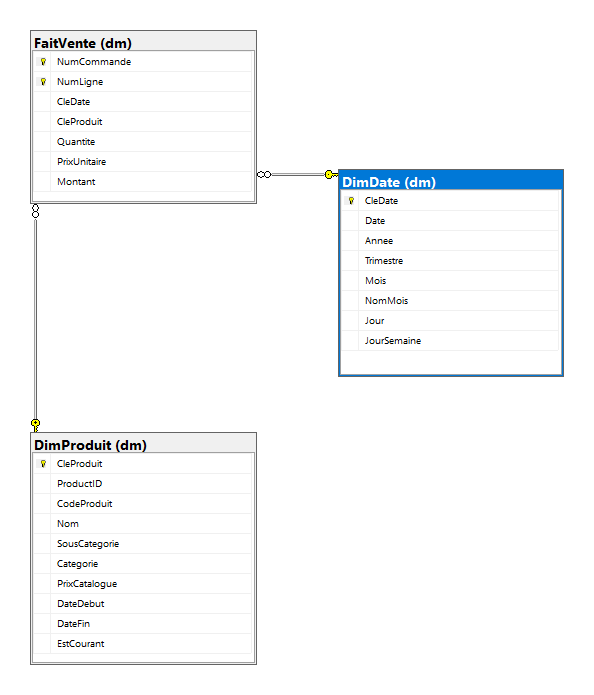
\includegraphics[width=\linewidth]{captures/C02_diagramme.png}
\captionof{figure}{Diagramme du data mart (C02).}
\end{minipage}

Une vente est rattachée à la version de produit valide à la date de la commande : \texttt{DateDebut} $\leq$ \texttt{OrderDate} et (\texttt{DateFin} $>$ \texttt{OrderDate} ou \texttt{DateFin} est NULL).

\subsection{Règles SCD}

\begingroup\small
\begin{tabularx}{\textwidth}{@{}>{\raggedright\arraybackslash}p{3.6cm}>{\raggedright\arraybackslash}p{2.3cm}X@{}}
\toprule
Élément & Règle & Traitement \\
\midrule
Prix catalogue & SCD type~2 & Chaque changement crée une nouvelle version \\
Sous-catégorie & SCD type~2 & Les ventes sont analysées selon la sous-catégorie valide à la date de la vente \\
Nom du produit & SCD type~1 & Un changement est une correction : la valeur est écrasée dans toutes les versions \\
Ligne de commande supprimée & --- & La ligne de fait est supprimée et le nombre de suppressions est journalisé \\
Ligne de commande modifiée & --- & La ligne de fait est mise à jour (quantité, montant) \\
Produit sans sous-catégorie & --- & Rattaché à la sous-catégorie et à la catégorie « Inconnu » \\
\bottomrule
\end{tabularx}
\endgroup

Date de début d'une nouvelle version : avec CDC, l'heure réelle du changement (obtenue à partir du LSN) ; avec Change Tracking, cette information n'existe pas et on utilise la date du chargement (conséquences discutées aux sections~4 et~5).

\subsection{Choix de conception}

\begingroup\small
\begin{tabularx}{\textwidth}{@{}c>{\raggedright\arraybackslash}p{5.2cm}X@{}}
\toprule
\# & Choix & Justification \\
\midrule
1 & \texttt{DateFin} = NULL pour la version courante (\texttt{EstCourant} = 1) & Sens clair : « pas encore terminée » (9999-12-31 était une alternative valable) \\
2 & \texttt{DateDebut} et \texttt{DateFin} en \texttt{DATETIME2(3)} & Dans la partie~2, les transactions sont séparées de quelques secondes : un type \texttt{DATE} ne les distinguerait pas \\
3 & Première version de chaque produit : \texttt{DateDebut} = 2010-01-01 & Les ventes anciennes (2011--2014) sont rattachées à une version, et l'ETL et l'ELT produisent la même valeur (test \texttt{EXCEPT}) \\
4 & \texttt{CleDate} = année $\times$ 10\,000 + mois $\times$ 100 + jour & Calculée directement à partir de la date, identique dans les deux chemins \\
5 & Prix et montants en \texttt{MONEY} ; \texttt{Decimal} en Python (jamais \texttt{float}) & Même type que la source ; un \texttt{float} introduirait des écarts d'arrondi qui fausseraient l'\texttt{EXCEPT} \\
6 & Clé de \texttt{FaitVente} = (\texttt{NumCommande}, \texttt{NumLigne}) & Retrouver la ligne en chargement incrémental ; lignage intégré (section~1.2) \\
7 & Noms de colonnes en français, sans accents & Cohérence avec l'énoncé \\
\bottomrule
\end{tabularx}
\endgroup

\texttt{Montant} $=$ \texttt{Quantite} $\times$ \texttt{PrixUnitaire} ; la remise (\texttt{UnitPriceDiscount}) n'est pas utilisée.

\subsection{Métadonnées}

\begingroup\small
\begin{tabularx}{\textwidth}{@{}>{\raggedright\arraybackslash}p{2.4cm}>{\raggedright\arraybackslash}p{4.8cm}X@{}}
\toprule
Type & Table ou source & Contenu \\
\midrule
Techniques & Requêtes sur \texttt{INFORMATION\_SCHEMA} et les vues \texttt{sys} (non saisies à la main) & Colonnes, types, clés et nombre de lignes des cinq tables sources \\
Métier & \texttt{meta.DictionnaireDonnees} (et \texttt{sp\_addextendedproperty}) & Définition métier des 25 colonnes du data mart \\
Lignage & \texttt{meta.MappingColonnes} & Tables et colonnes sources, règle de transformation : 25 lignes dans la base CDC, 44 dans la base CT (\texttt{dm} $\leftarrow$ \texttt{stg} et \texttt{stg} $\leftarrow$ AdventureWorks, « copie brute ») \\
Opérationnelles & \texttt{meta.JournalChargement} & Numéro d'exécution, méthode (ETL, ELT, CDC, CT), début, fin, lignes lues, insérées, mises à jour, supprimées, rejetées, statut, message \\
Contrôle & \texttt{meta.EtatCDC}, \texttt{meta.EtatCT} & Dernier LSN traité, dernière version Change Tracking traitée, pour chaque table source \\
\bottomrule
\end{tabularx}
\endgroup

La règle de \texttt{DateDebut} est documentée différemment dans les deux bases (heure du changement pour CDC, date du chargement pour CT). Le mapping et un extrait du dictionnaire figurent en annexe~A (C03).

%==========================================================================
\section{Comparaison ETL / ELT, chiffrée}
\todo{À compléter par Bekir Uzumcu : temps d'exécution, nombre de lignes de code, lieu des transformations, conservation des données brutes, ce qu'il faut relancer si une règle change.}

\section{Déroulement des chargements incrémentaux et difficultés rencontrées}
\todo{À compléter par Eray Aksoy et Bekir Uzumcu : ordre 06a $\rightarrow$ CDC $\rightarrow$ CT $\rightarrow$ 06b $\rightarrow$ CDC $\rightarrow$ CT, délai de capture du CDC, mises à jour de \texttt{SalesOrderHeader} par les déclencheurs, difficultés.}

\section{Tableau de comparaison CDC / Change Tracking}
\todo{À compléter par Eray Aksoy ; chaque ligne doit s'appuyer sur une observation de nos propres expériences.}

\begingroup\small
\begin{tabularx}{\textwidth}{@{}>{\raggedright\arraybackslash}p{6.2cm}XX@{}}
\toprule
Critère & CDC & Change Tracking \\
\midrule
Qu'est-ce qui est capturé ? (anciennes valeurs, nouvelles valeurs, seulement « la ligne a changé ») & & \\
L'heure du changement est-elle connue ? & & \\
Les deux changements de prix de P (partie~2) sont-ils visibles ? & & \\
À quelle version de P la vente du changement~8 est-elle rattachée ? & & \\
Quelles informations obtient-on pour une ligne supprimée ? & & \\
Faut-il SQL Server Agent ? & & \\
Que se passe-t-il si la durée de rétention est dépassée ? & & \\
Charge et stockage supplémentaires sur la source ? & & \\
Dans quels cas recommandez-vous chacun ? & & \\
\bottomrule
\end{tabularx}
\endgroup

\section{Résultats des tests}
\todo{À compléter par Eray Aksoy : résultats de \texttt{09\_tests.sql} dans chacun des deux data marts (capture C11).}

\section{Recommandation}
\todo{À rédiger ensemble : quelle combinaison (ETL ou ELT, CDC ou CT) recommandée à la direction d'Adventure Works, et pourquoi.}

\section{Déclaration de contribution}

\begingroup\small
\begin{tabularx}{\textwidth}{@{}>{\raggedright\arraybackslash}p{2.6cm}>{\raggedright\arraybackslash}p{3.2cm}X>{\raggedright\arraybackslash}p{2.2cm}@{}}
\toprule
Membre & Rôle & Contribution & Signature \\
\midrule
Erdem Ertan & Modélisation et métadonnées & Conception du data mart et du schéma \texttt{meta} (\texttt{01\_schema.sql}, \texttt{02\_metadonnees.sql}), règles SCD et choix de conception, diagramme (C02) et capture du mapping (C03), partie « article » de la présentation, sections 1 et 2 du rapport. & \\
\addlinespace
Bekir Uzumcu & ETL / ELT & \todo{à compléter} & \\
\addlinespace
Eray Aksoy & Capture des changements et tests & \todo{à compléter} & \\
\bottomrule
\end{tabularx}
\endgroup

\begin{thebibliography}{1}
\bibitem{mekterovic2011} I.~Mekterovi\'c, Lj.~Brki\'c, M.~Baranovi\'c, \emph{A Generic Procedure for Integration Testing of ETL Procedures}, Automatika, 52(2), 2011, p.~169--178.
\end{thebibliography}

%==========================================================================
\newpage
\section*{Annexe A --- Captures d'écran}

\begin{figure}[H]
  \centering
  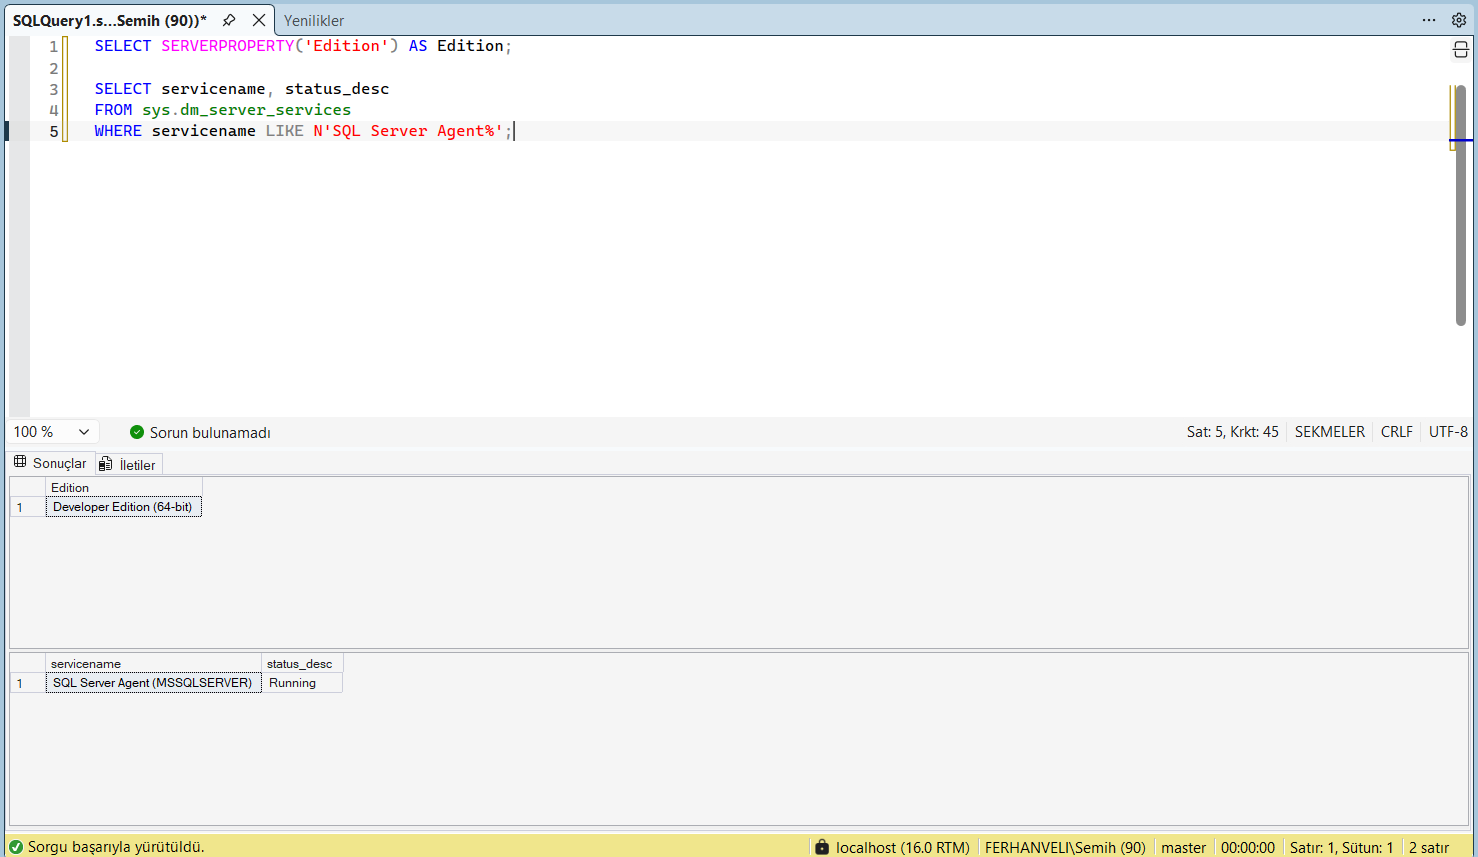
\includegraphics[width=0.8\textwidth]{captures/C01_environnement.png}
  \caption{C01 --- Environnement : édition de SQL Server (Developer) et état du service SQL Server Agent (\texttt{Running}).}
\end{figure}

\begin{figure}[H]
  \centering
  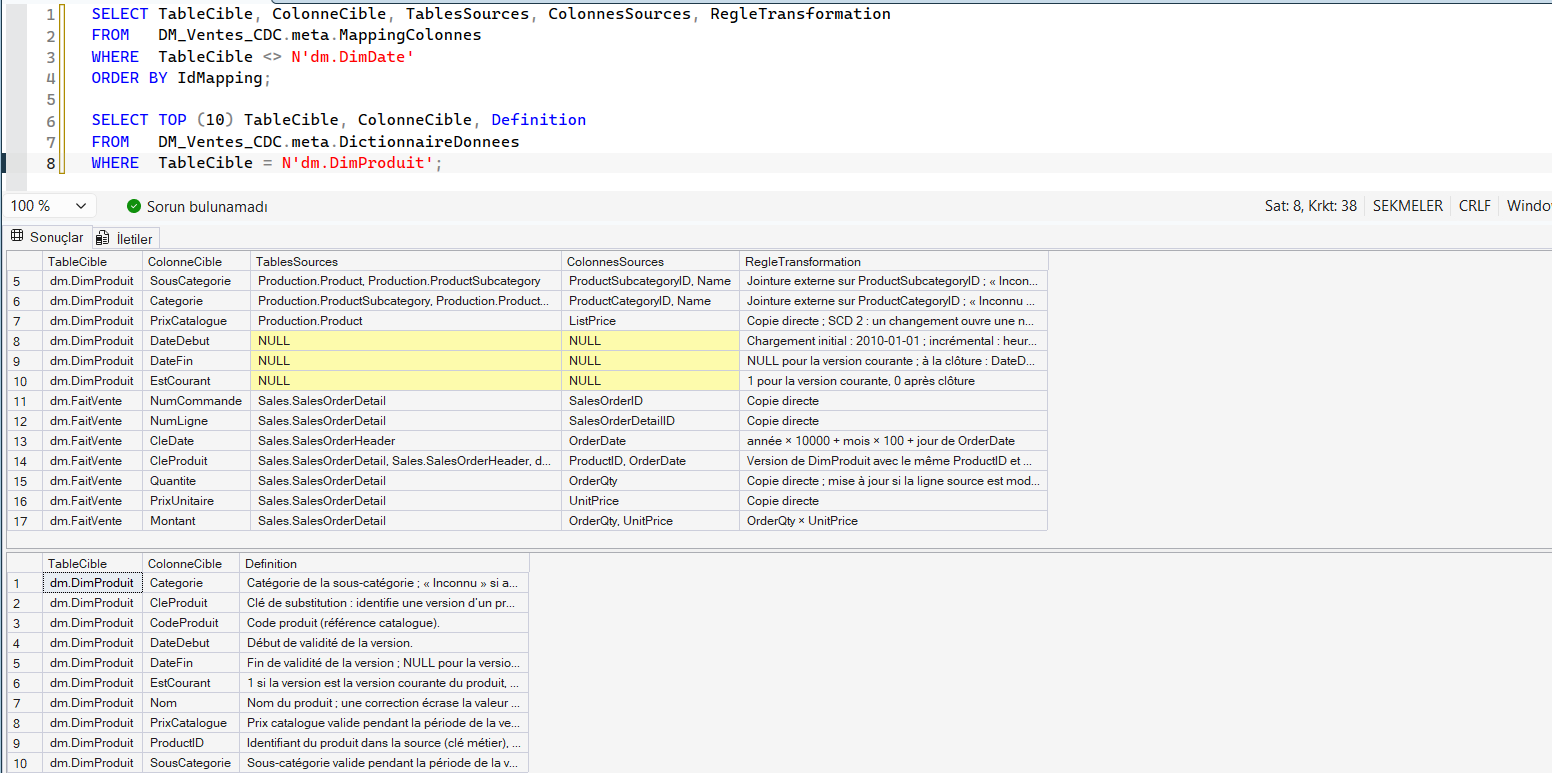
\includegraphics[width=0.95\textwidth]{captures/C03_mapping_dictionnaire.png}
  \caption{C03 --- Contenu de \texttt{meta.MappingColonnes} (hors \texttt{DimDate}) et extrait de \texttt{meta.DictionnaireDonnees} (\texttt{DimProduit}).}
\end{figure}

\end{document}
